% ============================================================
% PAGE 12-15 -- RESULTS
% ============================================================
\section{Results and Discussion}
\label{sec:results}

All numbers in this section were produced by the code accompanying this report;
the tables and plots are generated automatically from the measured data.

\subsection{Dataset Preparation}

The corpus consists of \numKernels\ C kernels in \numFamilies\ families
(Table~\ref{tab:corpus}). Each kernel is generated by sweeping the data type
(\texttt{float}/\texttt{double}), the problem size, the number of operands, the
access stride, the loop order or the dependence distance. Every kernel was
compiled with all \numConfigs\ configurations (\numCompiles\ compilations) and
executed; for each configuration the binary was run in five interleaved rounds
(\numRuns\ executions in total), and each execution reports the minimum of five
timed trials.

\begin{table}[H]
\centering
\caption{Composition of the loop-kernel corpus.}
\label{tab:corpus}
\small

\begin{tabular}{llcrr}
\toprule
\textbf{Family} & \textbf{Loop pattern} & \textbf{Depth} & \textbf{Kernels} & \textbf{Footprint (bytes)} \\
\midrule
\texttt{axpy} & vector update $y_i=\sum w_jx^{(j)}_i+\dots$ & 1 & 36 & $2^{13}$--$2^{24}$ \\
\texttt{cond} & loop with data-dependent branch & 1 & 16 & $2^{13}$--$2^{23}$ \\
\texttt{dot} & dot product / norm (FP reduction) & 1 & 18 & $2^{12}$--$2^{23}$ \\
\texttt{matmul} & matrix product, loop orders ijk/ikj/jki & 3 & 24 & $2^{14}$--$2^{20}$ \\
\texttt{recur} & first-order recurrence $a_i=f(a_{i-d})$ & 1 & 24 & $2^{13}$--$2^{23}$ \\
\texttt{stencil1d} & 3- and 5-point 1-D stencil & 1 & 16 & $2^{13}$--$2^{23}$ \\
\texttt{stencil2d} & 5-point 2-D Jacobi stencil & 2 & 8 & $2^{15}$--$2^{22}$ \\
\texttt{strided} & non-unit-stride gather $x[s\,i]$ & 1 & 20 & $2^{15}$--$2^{26}$ \\
\texttt{traverse2d} & 2-D row/column sums, copy, transpose & 2 & 20 & $2^{17}$--$2^{24}$ \\
\textbf{Total} &  &  & \textbf{182} &  \\
\bottomrule
\end{tabular}
\end{table}


\subsection{System Requirements}

\begin{table}[H]
\centering
\caption{System used for the experiments.}
\begin{tabular}{ll}
\toprule
\textbf{Component} & \textbf{Value}\\
\midrule
Processor & \cpuModel\ (AVX2 and AVX-512 available)\\
Cores available & \numCpus\\
RAM & \memGB\ GB\\
Operating System & Ubuntu 24.04 (Linux)\\
Compiler & \gccVersion\\
Programming Language & C (kernels), Python 3.12 (front end, ML)\\
Libraries & NumPy, pandas, scikit-learn\\
\bottomrule
\end{tabular}
\end{table}

\subsection{Evaluation Process}

The approach is evaluated with the following metrics. Let $T_c(L)$ be the time of
loop $L$ with configuration $c$, $\hat c(L)$ the predicted configuration, and
$c^{\star}(L)$ the fastest admissible configuration (oracle).

\subsubsection{Execution Time and Speed-up}

\[
S(L)=\frac{T_{O2}(L)}{T_{\hat c(L)}(L)} ,\qquad
\mathrm{GM}=\Big(\prod_{L} S(L)\Big)^{1/N}
\]

If the predicted configuration would change the numerical result, the safe baseline
\texttt{O2} is used instead (S = 1).

\subsubsection{Oracle Gain}

\[
G=\frac{\ln \mathrm{GM}_{\text{model}}}{\ln \mathrm{GM}_{\text{oracle}}}\times100
\]

\subsubsection{Regret}

\[
R=\frac{1}{N}\sum_L\left(\frac{T_{\hat c(L)}(L)}{T_{c^{\star}(L)}(L)}-1\right)\times100
\]

\subsubsection{Classification Metrics}

Accuracy and macro-averaged F1 over the \numConfigs\ classes are also reported.
They are less informative than speed-up because many configurations have almost the
same performance for a given loop.

\subsubsection{Validation Protocols}

\emph{Random 5-fold cross-validation} (repeated five times) measures interpolation
between similar loops. \emph{Leave-one-family-out} (LOFO) trains on eight families
and tests on the ninth, which measures generalisation to a new kind of loop and is
the stricter test.

\subsection{Measurement Noise}

The experiments ran on a shared virtual machine, and timings of the \emph{same} binary
vary from process to process (probably through physical-page placement and
cache conflicts). Across the five rounds, the baseline time of a kernel had a median
range of \noiseSpreadMedian\% (maximum minus minimum). Because the reported time is the
minimum over the rounds, the residual noise is smaller: comparing the minimum of the
odd rounds with the minimum of the even rounds gives a median difference of
\noiseSplitMedian\% (90th percentile \noiseSplitNinety\%). The 5\% tie tolerance of the
labelling rule is therefore of the order of the noise, but not above it for all kernels,
and some labels, especially among near-equivalent configurations, are uncertain.
This is a limitation of the experiment, discussed in Section~\ref{sec:limits}.

\subsection{Labels and Static Configurations}

Table~\ref{tab:labels} shows how often each configuration is the label and how a
\emph{static} choice of that configuration would perform over the whole corpus.
No static configuration is best for every kernel (the oracle is above all of them), which is the reason to learn the decision, but the aggressive configurations are close to the oracle on average.

\begin{table}[H]
\centering
\caption{Label distribution and performance of each \emph{static} configuration over all kernels (speed-up w.r.t.\ \texttt{O2}; a configuration that changes the numerical result is replaced by \texttt{O2}).}
\label{tab:labels}
\small
\resizebox{\textwidth}{!}{%
\begin{tabular}{lrrrrr}
\toprule
\textbf{Config} & \textbf{Label count} & \textbf{Label \%} & \textbf{GM speed-up} & \textbf{Within 5\% of best} & \textbf{Rejected} \\
\midrule
\texttt{O2} & 25 & 13.7 & 1.000 & 25 & 0 \\
\texttt{O3} & 6 & 3.3 & 1.054 & 23 & 0 \\
\texttt{O2\_unroll4} & 2 & 1.1 & 1.084 & 26 & 0 \\
\texttt{O2\_unroll8} & 2 & 1.1 & 1.109 & 29 & 0 \\
\texttt{O3\_native} & 65 & 35.7 & 1.512 & 92 & 0 \\
\texttt{O3\_unroll\_native} & 37 & 20.3 & 1.560 & 114 & 0 \\
\texttt{O3\_fast\_native} & 45 & 24.7 & 2.197 & 128 & 0 \\
\textbf{Oracle} & -- & -- & \textbf{2.316} & -- & -- \\
\bottomrule
\end{tabular}}
\end{table}


\begin{figure}[H]
\centering
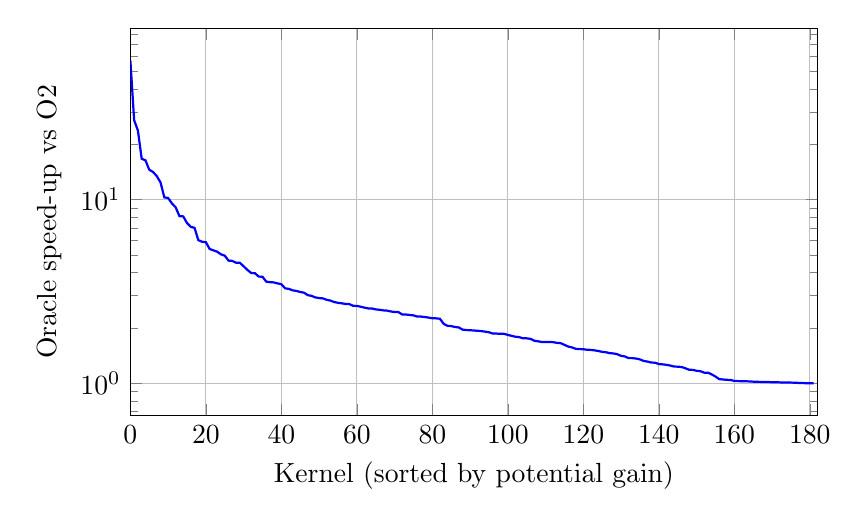
\begin{tikzpicture}
\begin{axis}[width=0.85\textwidth, height=6.5cm, xlabel={Kernel (sorted by potential gain)},
    ylabel={Oracle speed-up vs O2}, ymode=log, grid=major, xmin=0, xmax=182]
\addplot[thick, blue, no marks] coordinates {(0,57.256) (1,27.126) (2,23.777) (3,16.697) (4,16.376) (5,14.556) (6,14.146) (7,13.433) (8,12.393) (9,10.289) (10,10.210) (11,9.543) (12,9.080) (13,8.131) (14,8.106) (15,7.464) (16,7.109) (17,7.022) (18,6.018) (19,5.896) (20,5.866) (21,5.386) (22,5.293) (23,5.206) (24,5.037) (25,4.953) (26,4.655) (27,4.638) (28,4.532) (29,4.529) (30,4.336) (31,4.145) (32,3.986) (33,3.975) (34,3.810) (35,3.804) (36,3.575) (37,3.553) (38,3.541) (39,3.498) (40,3.464) (41,3.289) (42,3.265) (43,3.206) (44,3.182) (45,3.140) (46,3.113) (47,3.019) (48,2.991) (49,2.934) (50,2.910) (51,2.899) (52,2.848) (53,2.819) (54,2.768) (55,2.742) (56,2.725) (57,2.703) (58,2.699) (59,2.640) (60,2.638) (61,2.612) (62,2.581) (63,2.556) (64,2.553) (65,2.524) (66,2.513) (67,2.494) (68,2.486) (69,2.460) (70,2.442) (71,2.441) (72,2.369) (73,2.367) (74,2.354) (75,2.342) (76,2.307) (77,2.307) (78,2.294) (79,2.278) (80,2.259) (81,2.256) (82,2.245) (83,2.107) (84,2.055) (85,2.048) (86,2.024) (87,2.013) (88,1.959) (89,1.948) (90,1.945) (91,1.937) (92,1.931) (93,1.923) (94,1.910) (95,1.895) (96,1.866) (97,1.864) (98,1.859) (99,1.858) (100,1.834) (101,1.812) (102,1.792) (103,1.783) (104,1.757) (105,1.756) (106,1.745) (107,1.705) (108,1.692) (109,1.678) (110,1.678) (111,1.677) (112,1.674) (113,1.660) (114,1.653) (115,1.618) (116,1.584) (117,1.567) (118,1.540) (119,1.535) (120,1.532) (121,1.522) (122,1.519) (123,1.510) (124,1.498) (125,1.482) (126,1.475) (127,1.458) (128,1.453) (129,1.439) (130,1.410) (131,1.399) (132,1.370) (133,1.370) (134,1.363) (135,1.348) (136,1.322) (137,1.312) (138,1.296) (139,1.294) (140,1.272) (141,1.267) (142,1.260) (143,1.249) (144,1.233) (145,1.231) (146,1.226) (147,1.207) (148,1.185) (149,1.182) (150,1.169) (151,1.163) (152,1.142) (153,1.142) (154,1.118) (155,1.088) (156,1.053) (157,1.048) (158,1.044) (159,1.041) (160,1.030) (161,1.027) (162,1.026) (163,1.025) (164,1.023) (165,1.020) (166,1.018) (167,1.017) (168,1.017) (169,1.015) (170,1.013) (171,1.012) (172,1.011) (173,1.009) (174,1.009) (175,1.008) (176,1.007) (177,1.004) (178,1.003) (179,1.000) (180,1.000) (181,1.000)};
\end{axis}
\end{tikzpicture}
\caption{Best achievable speed-up over \texttt{O2} for each kernel (oracle).}
\label{fig:oracle}
\end{figure}


Figure~\ref{fig:oracle} shows the per-kernel gain that an oracle obtains over \texttt{O2}.
Many kernels gain from \texttt{-march=native}, because the machine supports AVX2 and
AVX-512 and the default \texttt{x86-64} target does not use them. Reductions
(\texttt{dot}) gain most from \texttt{-ffast-math}, which is consistent with the fact that
floating-point reductions can only be vectorised if the additions may be re-associated.
The other families show smaller but significant differences between the configurations.

\subsection{Performance of the Decision Models}

\begin{table}[H]
\centering
\caption{Comparison of decision models and static baselines. GM = geometric mean over kernels; ``Oracle gain'' is the share of the oracle's log-speed-up that is realised; ``Slow-downs'' counts kernels more than 5\% slower than \texttt{O2}.}
\label{tab:models}
\small
\resizebox{\textwidth}{!}{%
\begin{tabular}{llrrrrrr}
\toprule
\textbf{Model} & \textbf{Protocol} & \textbf{Acc.\ (\%)} & \textbf{Macro-F1} & \textbf{GM speed-up} & \textbf{Oracle gain (\%)} & \textbf{Regret (\%)} & \textbf{Slow-downs} \\
\midrule
Always -O2 & -- & 13.7 & 0.03 & 1.000 & 0 & 245.5 & 0 \\
Always -O3 & -- & 3.3 & 0.01 & 1.054 & 6 & 232.1 & 32 \\
Always -O3 -march=native & -- & 35.7 & 0.08 & 1.512 & 49 & 170.9 & 17 \\
Always -O3 -march=native -ffast-math & -- & 24.7 & 0.06 & 2.197 & 94 & 6.0 & 6 \\
Majority class & 5-fold CV & 35.7 $\pm$ 0.0 & 0.08 & 1.512 & 49 & 170.9 & 17 \\
Majority class & LOFO & 24.7 & 0.07 & 1.513 & 49 & 170.8 & 16 \\
Decision Tree & 5-fold CV & 60.7 $\pm$ 2.9 & 0.34 & 2.130 & 90 & 16.2 & 6 \\
Decision Tree & LOFO & 41.2 & 0.22 & 1.706 & 64 & 79.8 & 13 \\
Random Forest & 5-fold CV & 63.4 $\pm$ 1.0 & 0.38 & 2.221 & 95 & 4.9 & 6 \\
Random Forest & LOFO & 41.2 & 0.22 & 1.714 & 64 & 78.0 & 14 \\
Gradient Boosting & 5-fold CV & 60.2 $\pm$ 1.1 & 0.37 & 2.175 & 92 & 12.9 & 5 \\
Gradient Boosting & LOFO & 32.4 & 0.19 & 1.650 & 60 & 96.4 & 15 \\
k-NN & 5-fold CV & 66.5 $\pm$ 1.5 & 0.41 & 2.221 & 95 & 5.0 & 6 \\
k-NN & LOFO & 48.4 & 0.27 & 1.794 & 70 & 64.7 & 12 \\
\bottomrule
\end{tabular}}
\end{table}


Table~\ref{tab:models} and Figure~\ref{fig:speedup} compare the models with the static baselines. In random
cross-validation the learned models use the loop features well: the \selModel\ reaches \selAccCV\% accuracy and a
geometric-mean speed-up of \selGMCV, i.e.\ \selFracCV\% of the oracle gain (\oracleGM). Accuracy is only moderate
(macro-F1 \selFscoreCV) because several configurations perform within a few percent of each other; the speed-up is the
more relevant quantity.

The comparison with the \emph{best static configuration} is, however, sobering. Always compiling with
\texttt{-O3 -march=native -ffast-math} already gives \gmOFast, i.e.\ \fastFrac\% of the oracle gain, with a regret of
\fastRegret\% and \fastSlow\ slow-downs. The learned model (\selGMCV, regret \selRegretCV\%, \selSlowCV\ slow-downs) is
only marginally better in cross-validation. The reason is that on this processor, which has AVX2 and AVX-512 units,
the most aggressive flag set is the right choice for most of the kernels, so there is little left to decide. That static
choice is, however, not portable (it uses the instruction set of the build machine) and it relaxes IEEE floating-point
semantics; it passed the $10^{-3}$ checksum test on all kernels here, which does not prove that it is safe in general.

\begin{figure}[H]
\centering
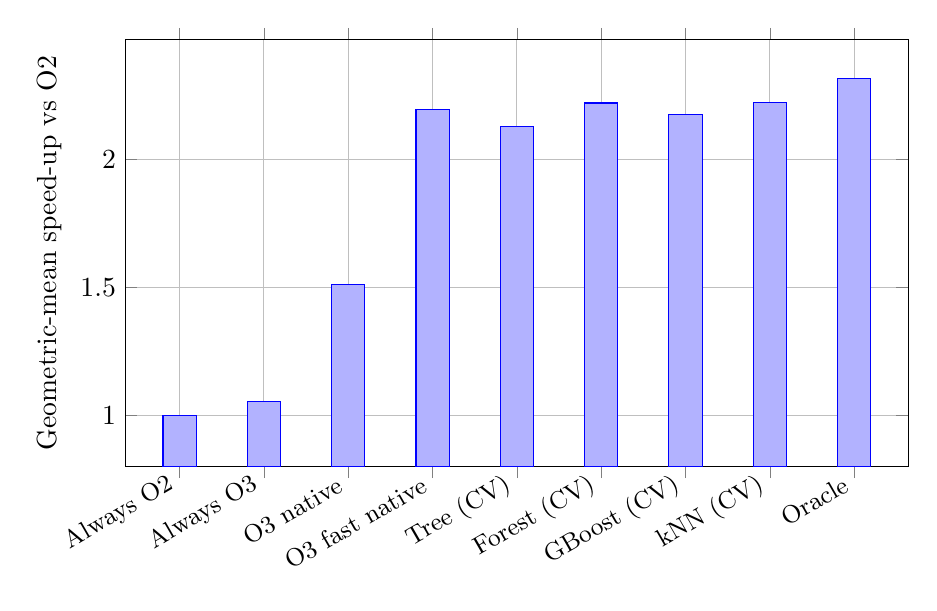
\begin{tikzpicture}
\begin{axis}[
    ybar, width=0.95\textwidth, height=7cm,
    ylabel={Geometric-mean speed-up vs O2},
    symbolic x coords={Always O2,Always O3,O3 native,O3 fast native,Tree (CV),Forest (CV),GBoost (CV),kNN (CV),Oracle},
    xtick=data, x tick label style={rotate=30,anchor=east,font=\small},
    ymin=0.8, 
    bar width=12pt,
    enlarge x limits=0.08,
    legend style={at={(0.5,1.03)},anchor=south,legend columns=-1,font=\small},
    grid=major]
\addplot coordinates {(Always O2,1.0000) (Always O3,1.0539) (O3 native,1.5122) (O3 fast native,2.1971) (Tree (CV),2.1300) (Forest (CV),2.2207) (GBoost (CV),2.1751) (kNN (CV),2.2215) (Oracle,2.3164)};

\end{axis}
\end{tikzpicture}
\caption{Geometric-mean speed-up over \texttt{O2} of the static configurations, the decision models (5-fold CV) and the oracle.}
\label{fig:speedup}
\end{figure}


Under leave-one-family-out the speed-up of the model falls to \selGMLOFO\ (\selFracLOFO\% of the oracle gain), the regret
rises from \selRegretCV\% to \selRegretLOFO\%, and the model is \emph{worse} than always choosing the aggressive
configuration (\gmOFast). Random splits overestimate the quality for new code because the corpus contains many close variants
of the same kernel. This is the main finding about the generalisation of the approach: with this corpus the model is not yet
reliable on a loop pattern that it has not seen.

\subsection{Portable Setting}

A more demanding decision arises when the program must run on any x86-64 machine and keep strict floating-point semantics.
The decision space is then restricted to \texttt{O2}, \texttt{O3}, \texttt{O2\_unroll4} and \texttt{O2\_unroll8}, and the
labels are recomputed from the same measurements with the same rule (Table~\ref{tab:portable}).

\begin{table}[H]
\centering
\caption{Portable setting: only the four IEEE-safe, non-native configurations (\texttt{O2}, \texttt{O3}, \texttt{O2\_unroll4}, \texttt{O2\_unroll8}) are allowed.}
\label{tab:portable}
\small
\resizebox{\textwidth}{!}{%
\begin{tabular}{llrrrrr}
\toprule
\textbf{Model} & \textbf{Protocol} & \textbf{Acc.\ (\%)} & \textbf{GM speed-up} & \textbf{Oracle gain (\%)} & \textbf{Regret (\%)} & \textbf{Slow-downs} \\
\midrule
Always -O2 & -- & 46.2 & 1.000 & 0 & 21.2 & 0 \\
Always -O3 & -- & 22.0 & 1.054 & 33 & 14.3 & 32 \\
Decision Tree & 5-fold CV & 51.9 & 1.088 & 53 & 9.0 & 5 \\
Decision Tree & LOFO & 37.4 & 1.012 & 7 & 19.6 & 8 \\
Random Forest & 5-fold CV & 52.1 & 1.102 & 60 & 7.3 & 7 \\
Random Forest & LOFO & 38.5 & 1.022 & 13 & 18.1 & 5 \\
k-NN & 5-fold CV & 57.1 & 1.108 & 64 & 6.6 & 6 \\
k-NN & LOFO & 43.4 & 1.039 & 23 & 15.8 & 3 \\
\textbf{Oracle} & -- & -- & \textbf{1.175} & 100 & 0.0 & 0 \\
\bottomrule
\end{tabular}}
\end{table}


Here the potential is smaller (oracle \pOracle), but the decision matters: always using \texttt{O3} gives \pOThree\ with
\pOThreeSlow\ kernels that become more than 5\% slower than \texttt{O2}. The \selModel\ reaches \pCV\ in cross-validation
(\pFracCV\% of the oracle gain) with \pSlowCV\ slow-downs on average, i.e.\ it keeps most of the benefit of \texttt{O3} while avoiding most of its
losses. Under leave-one-family-out it obtains \pLOFO\ (\pFracLOFO\% of the oracle gain) with \pSlowLOFO\ slow-downs: this is
slightly below the average speed-up of always using \texttt{O3}, but much safer.

\subsection{Per-Family Analysis}

\begin{table}[H]
\centering
\caption{Per-family geometric-mean speed-up over \texttt{O2} of the selected model (k-NN).}
\label{tab:family}
\small
\resizebox{\textwidth}{!}{%
\begin{tabular}{lrrrrrr}
\toprule
\textbf{Family} & \textbf{$n$} & \textbf{Oracle} & \textbf{Model (CV)} & \textbf{Model (LOFO)} & \textbf{Acc.\ CV (\%)} & \textbf{Acc.\ LOFO (\%)} \\
\midrule
\texttt{axpy} & 36 & 1.88 & 1.82 & 1.76 & 67 & 53 \\
\texttt{cond} & 16 & 5.02 & 4.98 & 1.29 & 81 & 6 \\
\texttt{dot} & 18 & 4.19 & 4.19 & 3.74 & 94 & 89 \\
\texttt{matmul} & 24 & 2.83 & 2.76 & 1.46 & 75 & 4 \\
\texttt{recur} & 24 & 1.38 & 1.26 & 1.27 & 54 & 42 \\
\texttt{stencil1d} & 16 & 1.73 & 1.67 & 1.67 & 50 & 81 \\
\texttt{stencil2d} & 8 & 2.26 & 2.23 & 2.21 & 25 & 75 \\
\texttt{strided} & 20 & 1.24 & 1.07 & 1.16 & 25 & 30 \\
\texttt{traverse2d} & 20 & 3.71 & 3.65 & 3.67 & 80 & 80 \\
\bottomrule
\end{tabular}}
\end{table}


\begin{figure}[H]
\centering
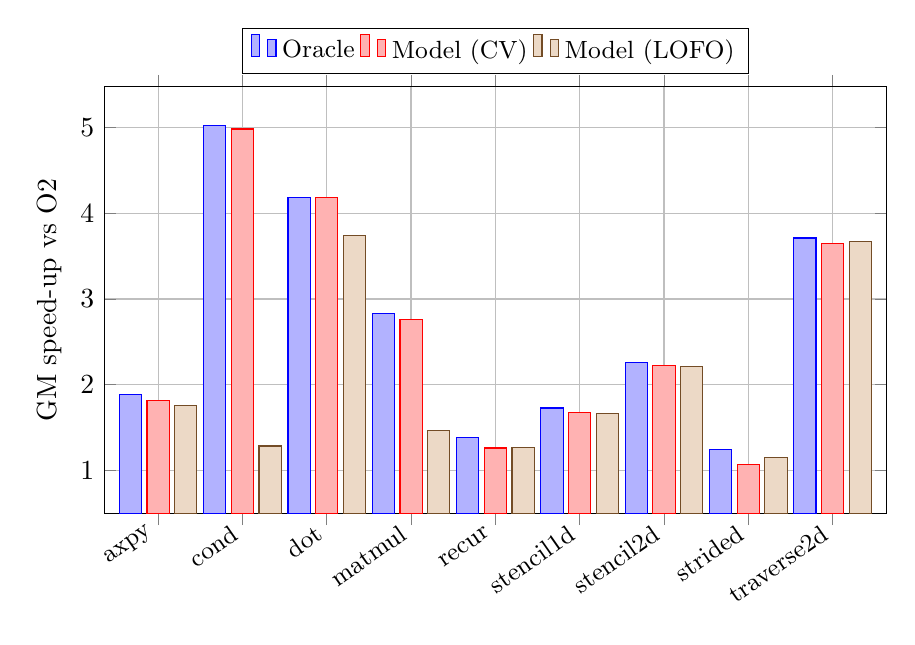
\begin{tikzpicture}
\begin{axis}[
    ybar, width=0.95\textwidth, height=7cm,
    ylabel={GM speed-up vs O2},
    symbolic x coords={axpy,cond,dot,matmul,recur,stencil1d,stencil2d,strided,traverse2d},
    xtick=data, x tick label style={rotate=35,anchor=east,font=\small},
    ymin=0.5, 
    bar width=8pt,
    enlarge x limits=0.08,
    legend style={at={(0.5,1.03)},anchor=south,legend columns=-1,font=\small},
    grid=major]
\addplot coordinates {(axpy,1.8813) (cond,5.0214) (dot,4.1862) (matmul,2.8279) (recur,1.3805) (stencil1d,1.7286) (stencil2d,2.2584) (strided,1.2434) (traverse2d,3.7099)};
\addplot coordinates {(axpy,1.8198) (cond,4.9817) (dot,4.1854) (matmul,2.7556) (recur,1.2621) (stencil1d,1.6731) (stencil2d,2.2253) (strided,1.0687) (traverse2d,3.6507)};
\addplot coordinates {(axpy,1.7556) (cond,1.2858) (dot,3.7438) (matmul,1.4649) (recur,1.2704) (stencil1d,1.6671) (stencil2d,2.2138) (strided,1.1561) (traverse2d,3.6741)};
\legend{Oracle,Model (CV),Model (LOFO)}
\end{axis}
\end{tikzpicture}
\caption{Per-family speed-up over \texttt{O2} for the k-NN: oracle, random-split cross validation, and leave-one-family-out.}
\label{fig:family}
\end{figure}


Table~\ref{tab:family} and Figure~\ref{fig:family} show that families with a clear structural signature
(\texttt{dot}, \texttt{traverse2d}, \texttt{matmul}, \texttt{cond}) are predicted nearly perfectly in
cross-validation. The \texttt{strided} family is the hardest: the best configuration depends on the
interaction of stride, cache size and the hardware prefetcher, which the static features describe only
roughly. In the leave-one-family-out test, \texttt{cond} and \texttt{matmul} lose most of their gain,
because no similar loop was in the training set: this indicates that the corpus must contain more
diverse loop patterns before the model can be trusted on new code. The families
\texttt{stencil1d}, \texttt{stencil2d}, \texttt{traverse2d} and \texttt{dot} transfer well because their
features resemble those of other families.

\subsection{Confusion Matrix and Feature Importance}

\begin{table}[H]
\centering
\caption{Confusion matrix of the k-NN (5-fold cross validation).}
\label{tab:confusion}
\scriptsize
\resizebox{\textwidth}{!}{%
\begin{tabular}{lrrrrrrr}
\toprule
\textbf{True $\backslash$ Pred} & \textbf{O2} & \textbf{O3} & \textbf{O2+unroll4} & \textbf{O2+unroll8} & \textbf{O3+native} & \textbf{O3+unroll+native} & \textbf{O3+fast+native} \\
\midrule
\textbf{O2} & 10 & 0 & 0 & 1 & 8 & 4 & 2 \\
\textbf{O3} & 1 & 2 & 0 & 0 & 2 & 1 & 0 \\
\textbf{O2+unroll4} & 0 & 0 & 0 & 0 & 0 & 2 & 0 \\
\textbf{O2+unroll8} & 1 & 0 & 0 & 0 & 1 & 0 & 0 \\
\textbf{O3+native} & 2 & 1 & 0 & 1 & 45 & 13 & 3 \\
\textbf{O3+unroll+native} & 5 & 0 & 1 & 0 & 6 & 22 & 3 \\
\textbf{O3+fast+native} & 0 & 0 & 0 & 0 & 5 & 3 & 37 \\
\bottomrule
\end{tabular}}
\end{table}


The confusion matrix (Table~\ref{tab:confusion}) shows that most errors are between neighbouring
aggressive configurations (for example \texttt{O3\_native} versus \texttt{O3\_unroll\_native}), whose
timing difference is small. Errors that choose a much slower configuration are rarer but produce the
slow-downs counted in Table~\ref{tab:models}.

\begin{figure}[H]
\centering
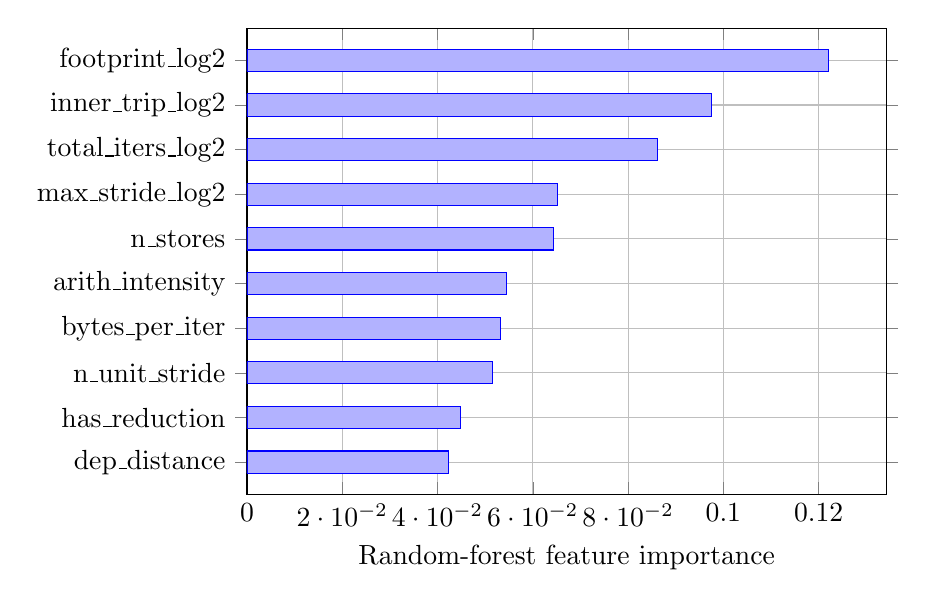
\begin{tikzpicture}
\begin{axis}[
    xbar, width=0.8\textwidth, height=7.5cm,
    xlabel={Random-forest feature importance},
    symbolic y coords={dep\_distance,has\_reduction,n\_unit\_stride,bytes\_per\_iter,arith\_intensity,n\_stores,max\_stride\_log2,total\_iters\_log2,inner\_trip\_log2,footprint\_log2},
    ytick=data, xmin=0, bar width=8pt, enlarge y limits=0.08, grid=major]
\addplot coordinates {(0.0423,dep\_distance) (0.0448,has\_reduction) (0.0515,n\_unit\_stride) (0.0532,bytes\_per\_iter) (0.0545,arith\_intensity) (0.0643,n\_stores) (0.0652,max\_stride\_log2) (0.0861,total\_iters\_log2) (0.0976,inner\_trip\_log2) (0.1220,footprint\_log2)};
\end{axis}
\end{tikzpicture}
\caption{Ten most important loop features.}
\label{fig:importance}
\end{figure}


Figure~\ref{fig:importance} shows that working-set size, trip counts and the largest memory stride
are the most important features. These are exactly the quantities that determine whether a loop is
bound by arithmetic, by cache or by memory bandwidth, and they are available from the
front end without running the program.

\subsection{Interpretable Rules}

A depth-5 decision tree trained on all data gives readable rules; the first levels are listed below
(\texttt{n\_stores}=0 identifies reductions, which are sent to \texttt{O3\_fast\_native}).

\lstinputlisting[language={},basicstyle=\ttfamily\scriptsize,numbers=none,lastline=26]{generated/decision_tree_rules.txt}

\subsection{Overhead of the Model}

Feature extraction takes about \featMs\ ms and prediction about \predMs\ ms per kernel, whereas a
single GCC compilation takes about \gccCompileMs\ ms on average. The decision is therefore of the same
order as, or cheaper than, one compiler run and is negligible compared with the search of an
iterative-compilation approach that compiles and runs every configuration (\numConfigs\ compilations per loop here).

\subsection{Sample Compiler Program}

The following C kernel (matrix product in the poor loop order j-k-i) is given to the advisor.
Note that this kernel is part of the training corpus, so the example illustrates the
tool and is not a test of generalisation.

\begin{lstlisting}
static DT A[M][M], B[M][M], C[M][M];   /* M = 96, DT = double */

DT kernel(int r)
{
    for (int j = 0; j < M; j++) {
        for (int k = 0; k < M; k++) {
            for (int i = 0; i < M; i++) {
                C[i][j] += A[i][k]*B[k][j];
            }
        }
    }
    return C[0][0];
}
\end{lstlisting}

\subsection{Lexical Analysis Output}

Token stream (first tokens of the loop, KIND:lexeme) for the kernel \texttt{cond\_double\_8192\_0p5\_1} printed by the scanner:

\lstinputlisting[language={},basicstyle=\ttfamily\small,numbers=none]{generated/tokens.txt}

\subsection{Three Address Code}

The loop nest of the same branchy kernel
(\texttt{if (x[i] > 0.5) y[i] = 0.5*x[i] + 0.1; else y[i] = 0.25*x[i];}) is lowered to the following
three-address code (before any optimisation; note the repeated loads of \texttt{x[i]}, which
common-subexpression elimination removes later):

\lstinputlisting[language={},basicstyle=\ttfamily\small,numbers=none]{generated/tac.txt}

\subsection{Advisor Output}

\lstinputlisting[language={},basicstyle=\ttfamily\scriptsize,numbers=none,firstline=1,lastline=5]{generated/predict_output.txt}
\lstinputlisting[language={},basicstyle=\ttfamily\scriptsize,numbers=none,firstline=28]{generated/predict_output.txt}

The feature vector, printed between these lines, shows the strides (96 elements for \texttt{C} and
\texttt{A}, i.e.\ a cache-hostile access), and the advisor selected \texttt{O2\_unroll4}, which was measured to be
faster than \texttt{-O2} for this kernel.

\subsection{Limitations and Threats to Validity}
\label{sec:limits}

\begin{itemize}
    \item \textbf{Single machine:} the labels depend on this processor. The large gains of the
    \texttt{native} configurations come from its AVX2/AVX-512 units; a different CPU requires re-labelling and re-training.
    \item \textbf{Synthetic corpus:} the kernels are small, regular HPC loops rather than whole applications, and similar
    kernels appear in several sizes. Random cross-validation is therefore optimistic, as the LOFO results show.
    \item \textbf{Timing noise:} on a shared virtual machine the residual noise (Section above) is comparable to the 5\% tie tolerance.
    \item \textbf{Numerical safety:} \texttt{-ffast-math} changes floating-point results. A configuration is only admissible if
    the checksum stays within a relative error of $10^{-3}$, which is a coarse test and is not a proof of correctness for other inputs.
    \item \textbf{Language subset:} the front end handles a C subset (affine subscripts, constant bounds, one function), not full C.
    \item \textbf{Portability:} binaries built with \texttt{-march=native} run only on processors with the same instruction set.
\end{itemize}

\newpage
